	\newpage
\section{Testowanie}	%5
%Opisujemy testy, sprawdzamy czy nie generuje błędów.
\subsection{Tworzenie nowego konta oraz logowanie do aplikacji}

Naszym celem jest utworzenie nowego konta użytkownika a następnie zalogowanie się do aplikacji przy pomocy nowo utworzonego konta.

\begin{figure}[!htb]
	\begin{center}
		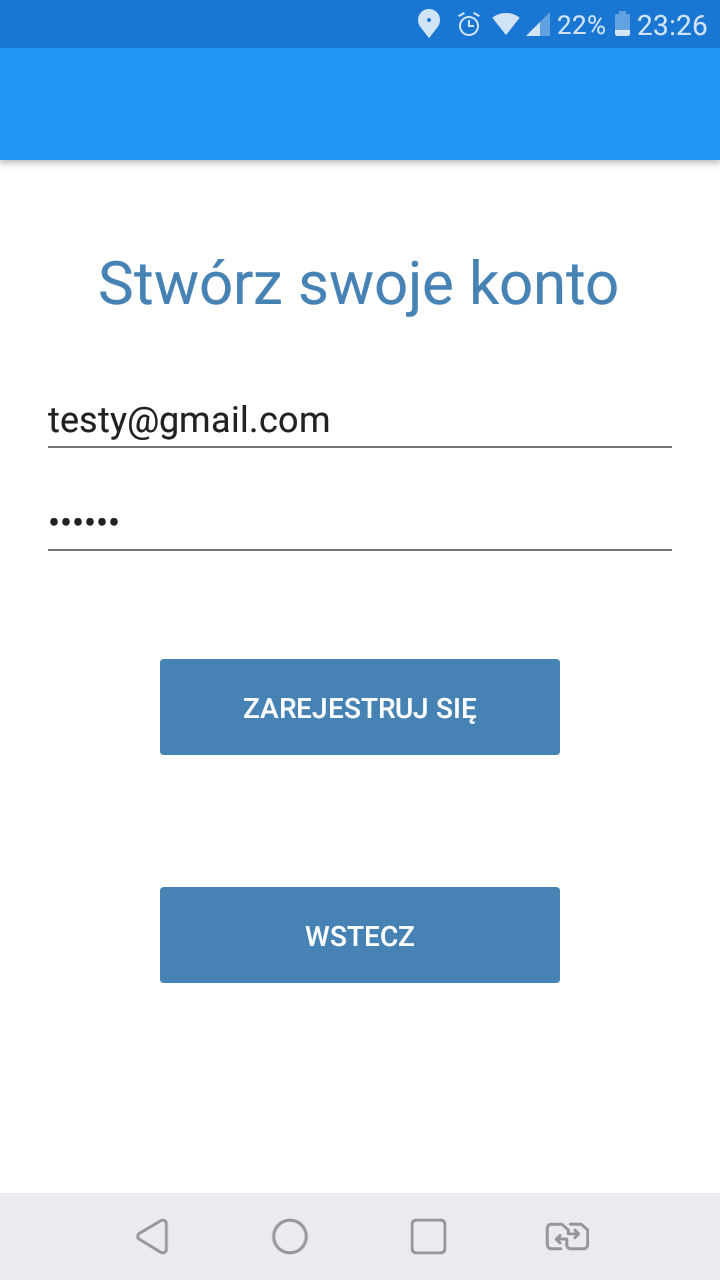
\includegraphics[width=4cm]{rys/ZZkonto.png}
		\caption{Tworzenie nowego konta}
		\label{rys:rysunek029}
	\end{center}
\end{figure}

Wpisujemy poprawny adres E-mail oraz hasło składające się z co najmniej sześciu znaków jak to jest pokazane na rysunku 5.1 a następnie klikamy przycisk zarejestruj się.

\begin{figure}[!htb]
	\begin{center}
		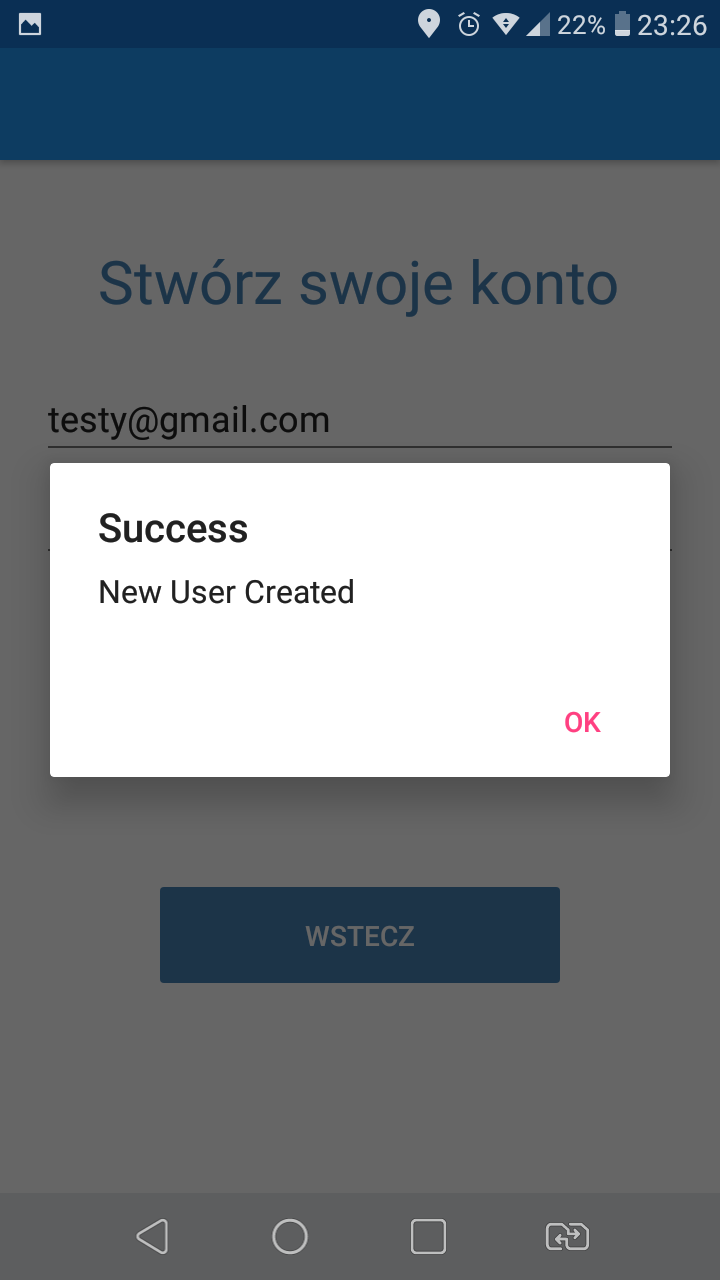
\includegraphics[width=4cm]{rys/ZZkonto2.png}
		\caption{Informacja o utworzeniu konta}
		\label{rys:rysunek030}
	\end{center}
\end{figure}

Po kliknięciu przycisku zarejestruj się otrzymujemy informacje, że tworzenie nowego konta przebiegło pomyślnie jak widać na rysunku 5.2.

\begin{figure}[!htb]
	\begin{center}
		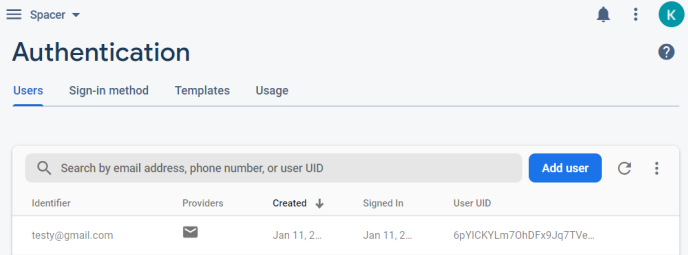
\includegraphics[width=12cm]{rys/ZZauth.png}
		\caption{Nowe konto w bazie danych}
		\label{rys:rysunek031}
	\end{center}
\end{figure}

Na rysunku 5.3 widzimy, że nowy użytkownik został dodany w bazie danych Google Firebase co oznacza, że powinna być możliwość zalogowania się na jego konto.

\begin{figure}[!htb]
	\begin{center}
		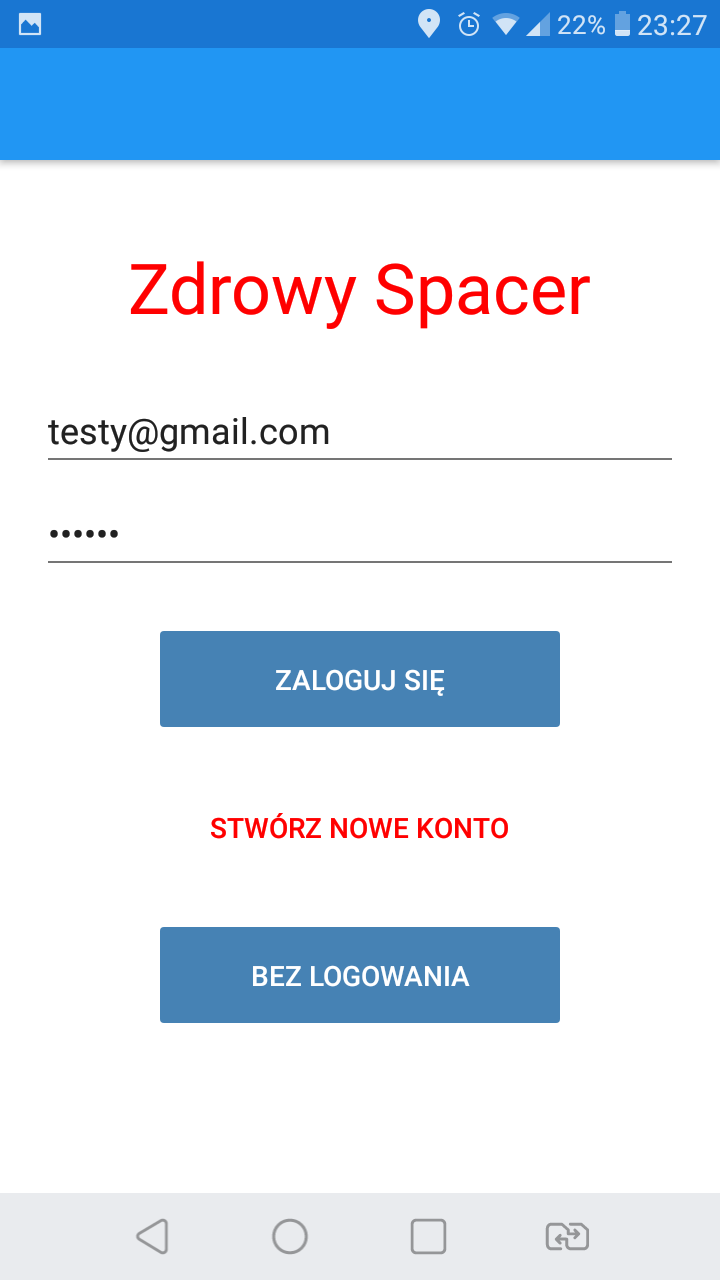
\includegraphics[width=4cm]{rys/ZZlog.png}
		\caption{Logowanie na utworzone konto}
		\label{rys:rysunek032}
	\end{center}
\end{figure}

Na stronie logowania jak widać na rysunku 5.4 wpisujemy E-mail i hasło takie samo jak podczas zakładania konta. Następnie klikamy przycisk zaloguj się.

\begin{figure}[!htb]
	\begin{center}
		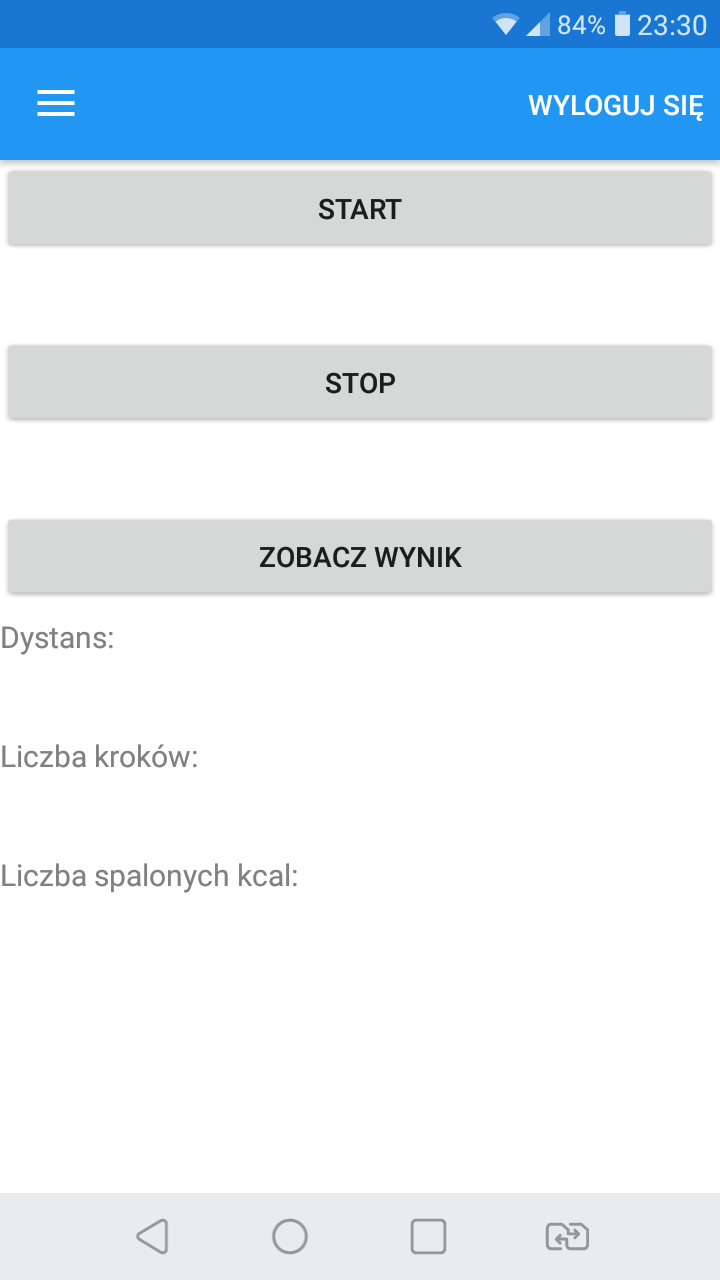
\includegraphics[width=4cm]{rys/ZZsg.png}
		\caption{Widok po zalogowaniu}
		\label{rys:rysunek033}
	\end{center}
\end{figure}

Jak widać na rysunku 5.5 logowanie przebiegło pomyślnie i zostaliśmy przeniesieni na stronę główną aplikacji.

\subsection{Test działania geolokalizacji i geokodowania na stronie głównej}

Celem naszego testu jest sprawdzenie czy po kliknięciu przycsków aplikacja wykonuje oczekiwane przez nas działania. Przyciski start i stop powinny zwracać nam informacje naszym obecnym adresie pobieranym w momencie klikania danego przycisku. Przycisk zobacz wynik powinien wyświetlić nam wyniki czyli przebyty dystans, liczbę kroków i liczbę spalonych kalorii.

\begin{figure}[!htb]
	\begin{center}
		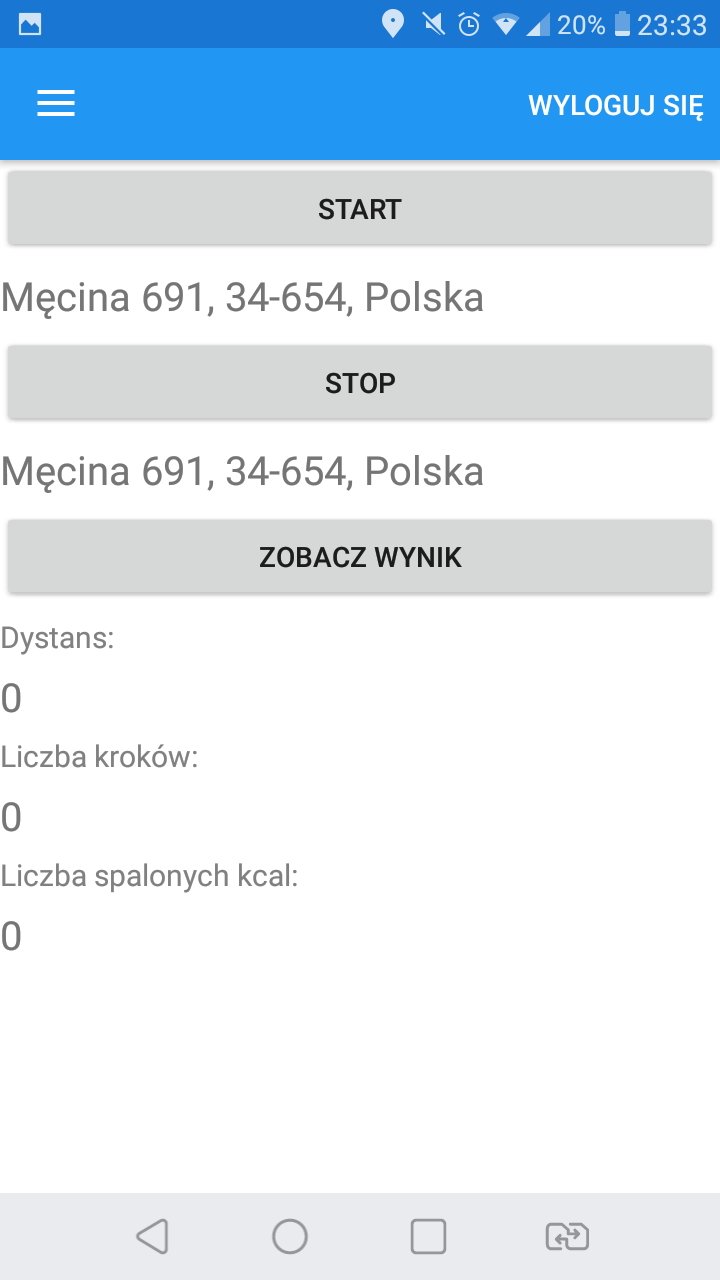
\includegraphics[width=4cm]{rys/ZZZ.png}
		\caption{Wyniki}
		\label{rys:rysunek034}
	\end{center}
\end{figure}

Na rysunku 5.6 pokazany jest wynik końcowy po użyciu wszystkich trzech przycisków. W momencie, gdy zaczynamy spacer naciskamy przycisk start a aplikacja wypisuje nam obecną lokalizację. Po zakończeniu spaceru naciskamy przycisk stop, aplikacja podaje nam adres końcowy. Naciskamy przycisk zobacz wyniki i otrzymujemy przebyty dystans, liczbę wykonanych kroków i liczbę spalonych kalorii. Pokazany dystans zgadza się z rzeczywistą odległością jaką przebyliśmy.

\subsection{Test działania mapy}

Nasza mapa powinna pokazywać miejsce w którym znjaduje się użytkownik za pomocą wskażnika. Po kliknięciu przycisku wybierz miejsce docelowe powinniśmy zostać przeniesieni do Google Maps, gdzię będzie możliwość wyznaczenia trasy poprzez wpisanie naszego celu.

\begin{figure}[!htb]
	\begin{center}
		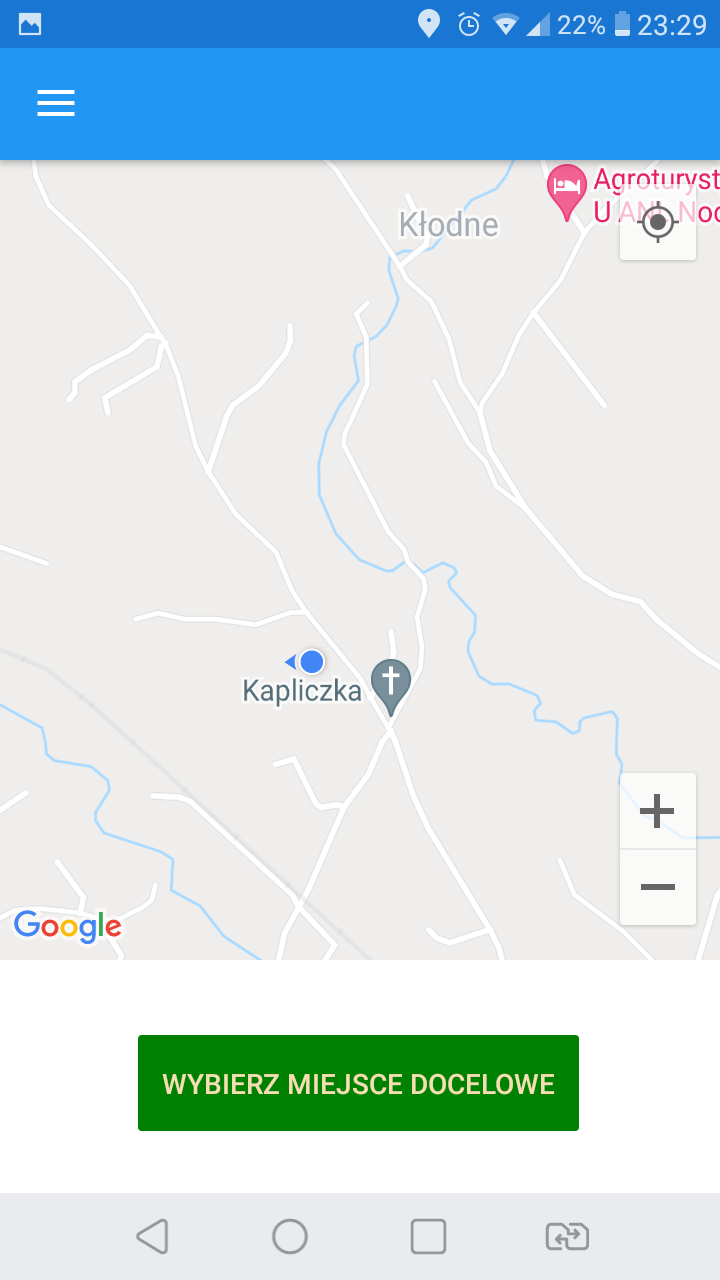
\includegraphics[width=3cm]{rys/ZZmapa.png}
		\caption{Mapa z lokalizacją}
		\label{rys:rysunek035}
	\end{center}
\end{figure} 

Jak widać na rysunku 5.7 mapa pokazuje naszą obecną lokalizację za pomocą wskaźnika. Wyznaczona lokalizacja jest zgodna z naszym realnym położeniem.

\begin{figure}[!htb]
	\begin{center}
		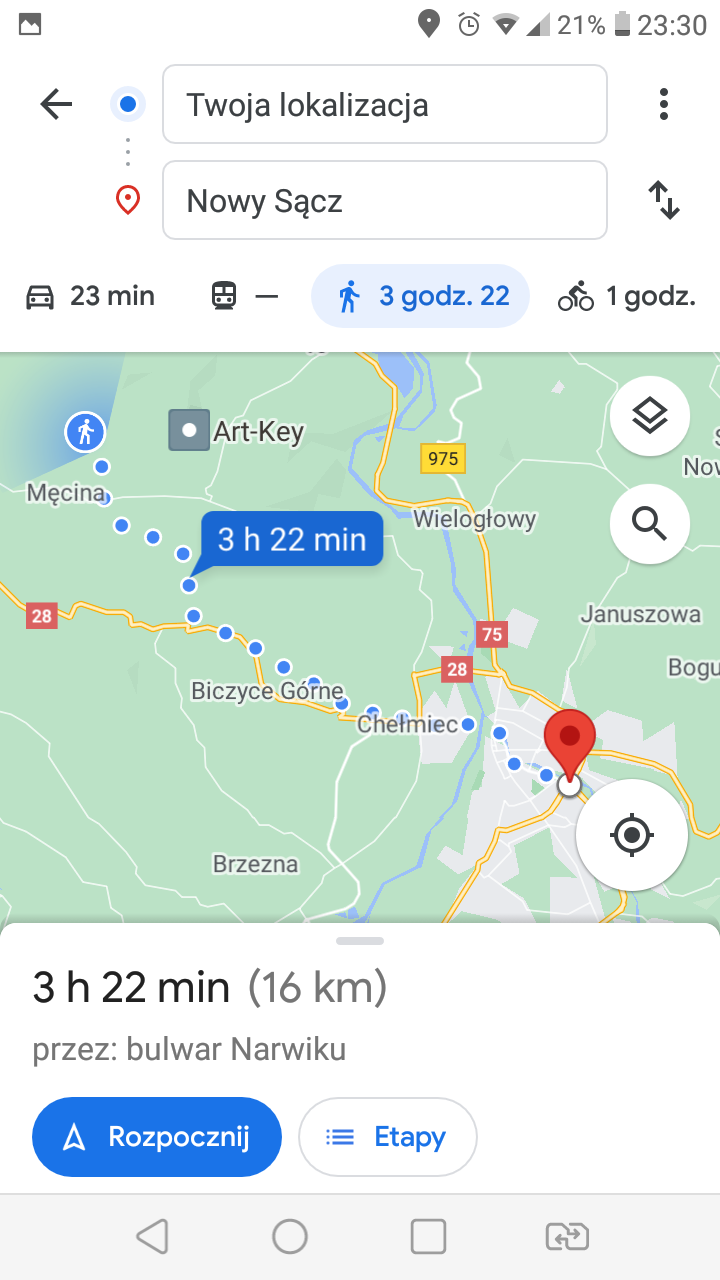
\includegraphics[width=3cm]{rys/ZZgm.png}
		\caption{Google Maps}
		\label{rys:rysunek036}
	\end{center}
\end{figure}

Po kliknięciu przycisku wybierz miejsce docelowe zostajemy przeniesieni do Google Maps, tam wpisujemy nasze miejsce docelowe i jak to jest pokazane na rysunku 5.8 otrzymujemy wyznaczoną trasę od naszego miejsca pobytu do miejsca docelowego.

\subsection{Obsługa aparatu i dodawanie zdjęcia z galerii}

Celem testu jest otwarcie aparatu z poziomu aplikacji i wykonanie zdjęcia, które następnie powinno zostać wyświetlone na stronie. Potem sprawdzimy możliwość zamiany tego zdjęcie na inne wybrane z galerii.

\begin{figure}[!htb]
	\begin{center}
		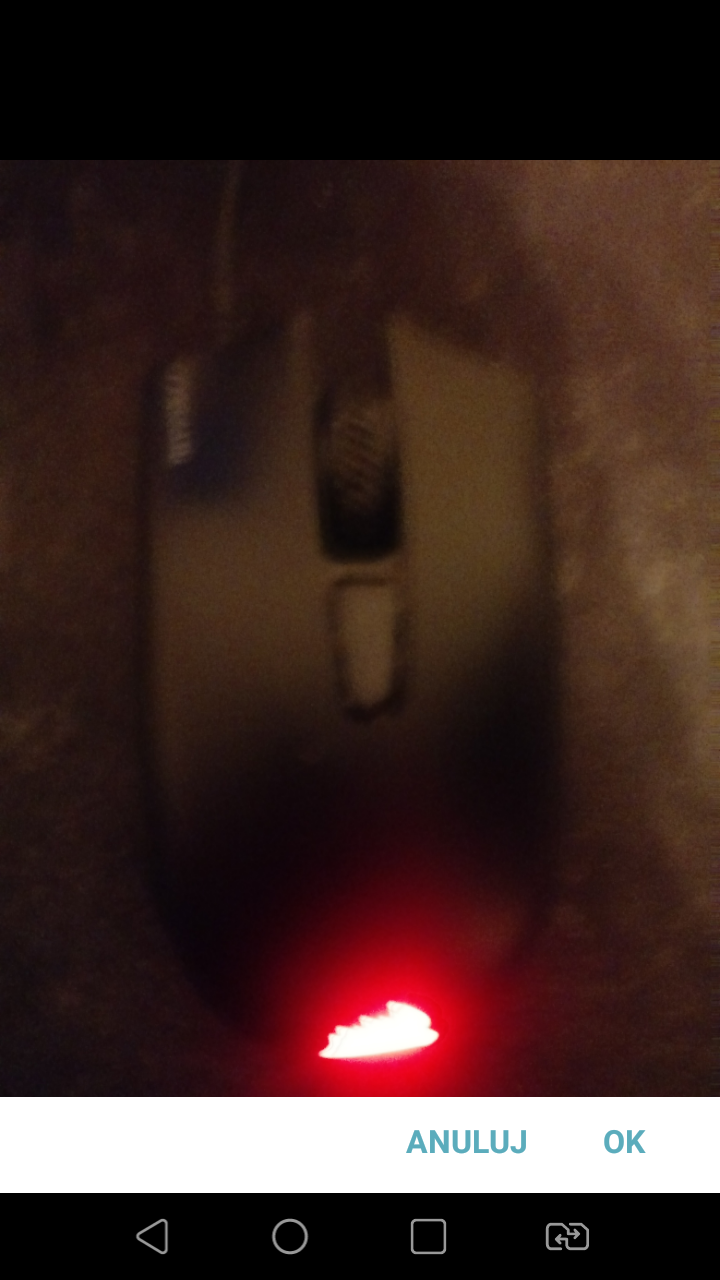
\includegraphics[width=3cm]{rys/ZZfoto.png}
		\caption{Wykonanie zdjęcia}
		\label{rys:rysunek037}
	\end{center}
\end{figure}

Po naciśnięciu przycisku zrób zdjęcie otwiera się nasz aparat z ustawioną domyślnie kamerą tylną aparatu. Po zrobieniu zdjęcia możemy je zatwierdzić klikając ok co widać na rysunku 5.9.

\begin{figure}[!htb]
	\begin{center}
		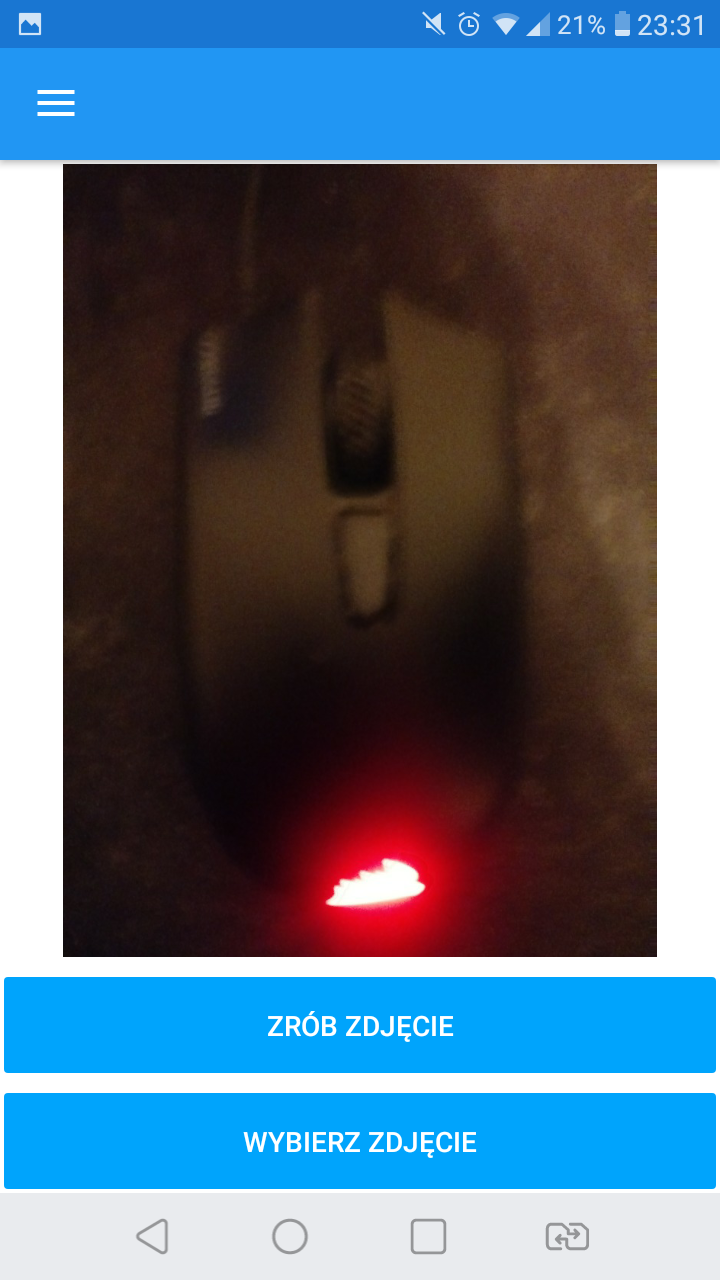
\includegraphics[width=3cm]{rys/ZZfoto2.png}
		\caption{Wyświetlenie zdjęcia}
		\label{rys:rysunek038}
	\end{center}
\end{figure}

Na rysunku 5.10 widać, że zdjęcie zostało poprawnie dodane na stronie w aplikacji.

\begin{figure}[!htb]
	\begin{center}
		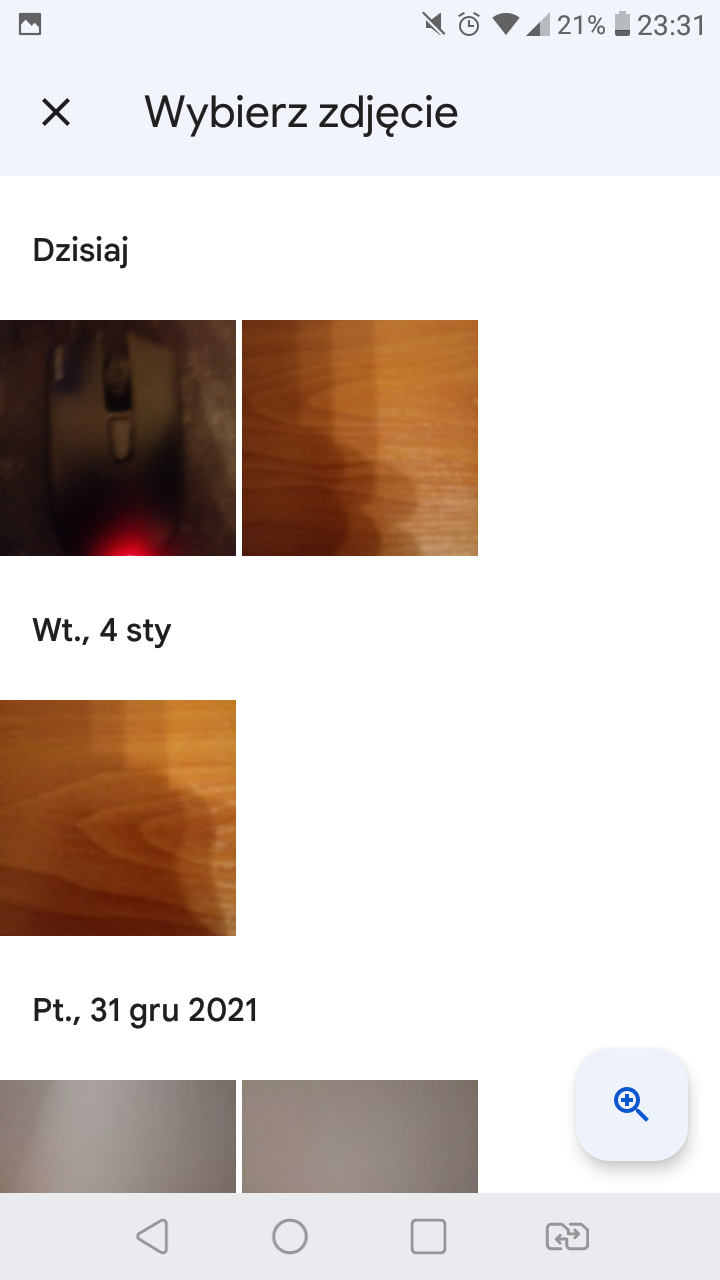
\includegraphics[width=4cm]{rys/ZZfoto3.png}
		\caption{Wybieranie zdjęcia z galerii}
		\label{rys:rysunek039}
	\end{center}
\end{figure}

Po kliknięciu przycisku wybierz zdjęcie otwiera się nasza galeria jak to jest pokazane na rysunku 5.11 w której możemy obejrzeć wykonane przez nas wcześniej zdjęcia. Wybieramy jedno z wcześniejszych zdjęć aby widzieć je w naszej aplikacji.

\begin{figure}[!htb]
	\begin{center}
		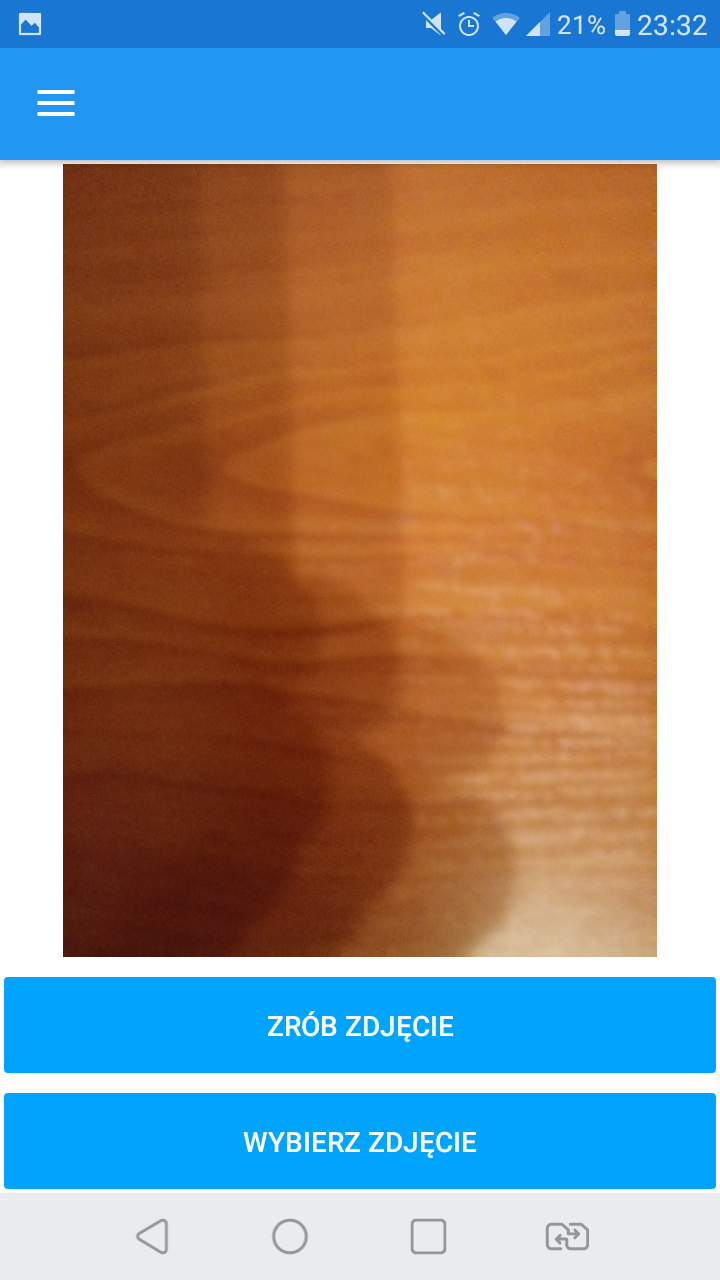
\includegraphics[width=4cm]{rys/ZZfoto4.png}
		\caption{Nowe zdjęcie}
		\label{rys:rysunek0340}
	\end{center}
\end{figure}

Jak widać na rysunku 5.12 zdjęcie zostało zmienione na to, które wybraliśmy z naszej galerii.

